\chapter{Actions}
\label{chp:actions}
Het laatste communicatietype van ROS 2 is actions. Action communicatie bestaat uit de communicatierollen \textit{action server} en \textit{action client}. Actions servers zijn een soort service servers met het grote verschil dat een action server feedback geeft aan de action client terwijl hij de request uitvoert. De action-communicatie is afgebeeld in figuur \ref{fig:action_node}. We zien daar dat een action eigenlijk bestaat uit \'e\'en topic en twee services.

Om een actie te starten stuurt de action client via de goal service een goal request. De action server reageert hier op met een \textit{accept} of met een \textit{reject}. Als de goal request is geaccepteerd, dan gaat de action server de goal uitvoeren en geeft tijdens het uitvoeren feedback over het uitvoeren van de actie aan de action client. Als de actie klaar is of gecanceld wordt, dan stuurt de action server het resultaat terug naar de action client. In tegenstelling tot bij services kunnen acties voortijdig gestopt worden. 

Als we naar afbeelding \ref{fig:action_node} kijken lijkt het alsof we ons zorgen moeten maken over twee services en een topic. Gelukkig neemt ROS 2 deze zorgen voor ons weg. Actions worden gezien als 1 communicatiestructuur en er zijn maar 3 berichten die we zelf moet definiëren: \textit{request}, \textit{result} en \textit{feedback}. Net als bij services moeten we de structuur van deze berichten vastleggen.  Bij actions leggen we deze structuur vast in een .action-bestand.

\begin{figure}[ht]
\begin{center}
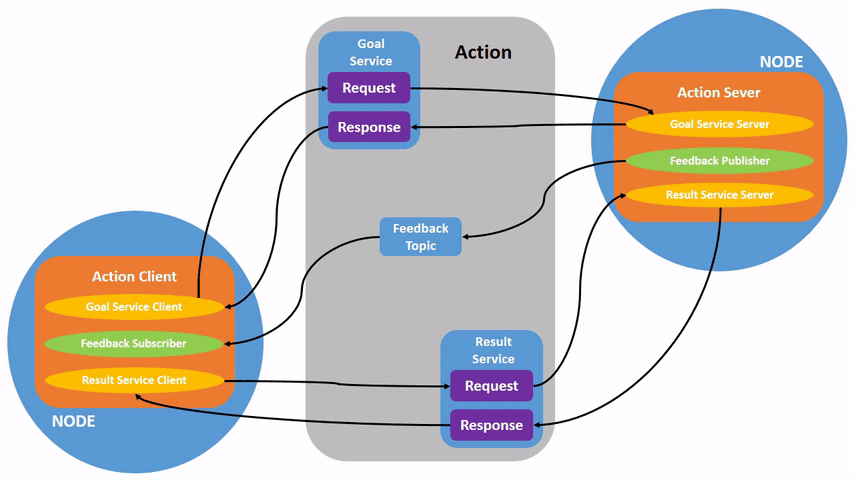
\includegraphics[scale=0.7]{Pictures/Action-SingleActionClient.png}\\
\end{center}
\caption{Action Node en een client node. {\tiny (afbeelding van ros.org\cite{ROSactionserver})}}\label{fig:action_node}
\end{figure}


\section{Action message structure}
\label{sec:action_message_structure}
Net als bij services moet de structuur van de berichten aangeven worden. Dit doen we in een .action-bestand en wordt in de ROS documentatie een `action' genoemd. In deze reader verwijzen we er naar met de term `action message structure'. In de action message structuur staan de parameters van de \textit{goal request}, van de \textit{result} en van de \textit{feedback}. In het bestand zijn deze onderdelen gescheiden door middel van drie gedachtenstreepjes (-)\footnote{zie: https://nl.wikipedia.org/wiki/Gedachtestreepje}. Met eerst de goal request, daarna de result en als laatste de structuur van de feedback. In codevoorbeeld \ref{code:template-action-bestand} zien we de template voor een action message structure. In codevoorbeeld \ref{code:action-fib-struct} zien we een uitgewerkte action message structure waarbij de goal request bestaat uit een int32, de result uit een vector<int32> en de feedback uit een vector<int32>. Net als bij services en topics beschrijven we per message een struct, dus we kunnen ook meerdere (verschillende) types toekennen aan \'e\'en bericht. 

\begin{lstlisting}[language=C++, caption={Template van een .action-bestand}, firstnumber=0, label={code:template-action-bestand}]
# Goal request
---
# Result
---
# Feedback
\end{lstlisting}

\begin{lstlisting}[language=C++, caption={Het .action-bestand voor een fibonacci-action server.}, firstnumber=0, label={code:action-fib-struct}]
int32 order
---
int32[] sequence
---
int32[] partial_sequence
\end{lstlisting}

\noindent De mogelijke types die kunnen worden gebruikt in de action message structure zijn te vinden op:
\begin{center}
    \url{https://index.ros.org/doc/ros2/Concepts/About-ROS-Interfaces/}
\end{center}

\noindent Net zoals het message type van de publishers/subscribers (zie sectie \ref{sec:message_types}) en de request and response structure van services (zie sectie \ref{sec:srv_messages}) is het mogelijk de action message structure binnen de package te plaatsen, maar ook om deze buiten de package te plaatsen. 

\noindent \textbf{Let op:} Bij het maken van een \textit{.action}-bestand is het verplicht in de naamgeving PascalCase\footnote{zie \url{https://nl.wikipedia.org/wiki/CamelCase}} te gebruiken. ROS zet de \textit{.action} om naar een \textit{.hpp}-bestand met de naam in snake\_case \footnote{zie: \url{https://en.wikipedia.org/wiki/Snake_case}}, waarbij tussen elke kleine letter en hoofdletter van de PascalCase naamgeving nu een onderstrepingsteken (\_) \footnote{ook wel bekent als \textit{underscore}. Zie \url{https://nl.wikipedia.org/wiki/Underscore}} staat. Bijvoorbeeld de action message structure beschreven in \textit{MyCustomAction.action} wordt geïncludeerd met: 
\begin{lstlisting}[language=C++, caption={}, firstnumber=0, label={}]
#include "path/to/folder/my_custom_action.hpp".
\end{lstlisting}

\noindent In sectie \ref{sec:action_meer_bronnen} staan meer bronnen over action message structure. In deze bronnen staat ook hoe je .action-bestanden toevoegd aan je package en hoe je ze vanuit een andere package includeert. 

\section{Action Server}
Een node noemen we een \textit{action server} als het een membervariabele van het type \textit{rclcpp\_action::Server<T>} heeft. Om historische redenen zitten de benodigdheden voor action server en client niet in rclcpp, maar in \textit{rclcpp\_action}. Deze includeren we met:

\begin{lstlisting}[language=C++, caption={}, firstnumber=0, label={}]
#include "rclcpp_action/rclcpp_action.hpp"
\end{lstlisting}

\noindent Met rclcpp\_action kunnen we vervolgens een action server declareren.
Bijvoorbeeld de action server \textit{action\_server\_} met de action message structure \textit{custom\_interfaces::action::Fibonacci}:

\begin{lstlisting}[language=C++, caption={}, firstnumber=0, label={}]
// 'using' allows us to use a shorter word for long types:
using FibAction = custom_interfaces::action::Fibonacci;
// [...]
rclcpp_action::Server<FibAction>::SharedPtr action_server_;"
\end{lstlisting}

Een action server moet drie typen berichten afhandelen: \textit{goal request}, \textit{cancel request} en \textit{accept and execute}. Bij elk bericht hoort ook een taak. De action server moet na het ontvangen van een goal request of een cancel request het verzoek accepteren of weigeren. Bij de ontvangst van een \textit{accept and execute} bericht moet de action server het uitvoeren van de goal starten. Tijdens het uitvoeren van de goal kan de action server feedback sturen naar de action client. Als de goal behaald is of als de goal wordt gecanceld wordt het resultaat gestuurd naar de action client.

Bij het initialiseren van de action server moeten we voor elk type bericht een functie toekennen die het bericht afhandelt. Deze functies hebben verplichte parameters die we bij het initialiseren binden met \textit{std::placeholders}. Het initialiseren doen we met de template-functie \textit{rclcpp\_action::create\_server<T>()} die als template de action message structure heeft. De complete initialisatie van de action server \textit{action\_server\_} in de class \textit{FibActionServer} met de functie \textit{handle\_goal} voor het afhandelen van de goal request, de functie \textit{handle\_cancel} voor het afhandelen van de cancel request en de functie \textit{handle\_accepted} voor het afhandelen van de goal acceptatie en executie ziet er uit als:

\begin{lstlisting}[language=C++, caption={Initialisatie van de action server \textit{action\_sever\_}.}, firstnumber=0, label={code:initialisatie_action_server}]
using namespace std::placeholders;
// 'using' allows us to use a shorter word for long types:
using FibAction = custom_interfaces::action::Fibonacci;
// [...]
this->action_server_ = rclcpp_action::create_server<FibAction>(
    this,
    "fibonacci",
    std::bind(&FibActionServer::handle_goal, this, _1, _2),
    std::bind(&FibActionServer::handle_cancel, this, _1),
    std::bind(&FibActionServer::handle_accepted, this, _1));
\end{lstlisting}

De functies die worden gebonden in tijdens de initialisatie van een \textit{rclcpp\_action::create\_server} hebben net als de functies bij subscribers, service server en service client verplichte parameters en return types. Om de lezer daar bewust van te maken laten we de functie declaraties zien van de gebonden functies in codevoorbeeld \ref{code:initialisatie_action_server}. In de volgende secties bekijken we de inhoud van deze functies.

\begin{lstlisting}[language=C++, caption={De \textit{action\_server\_} functies die de berichten afhandelen.}, firstnumber=0, label={code:action_server_functies}]
// 'using' allows us to use a shorter word for these long types:
using FibAction = custom_interfaces::action::Fibonacci;
using GoalHandleFib = rclcpp_action::ServerGoalHandle<FibAction>;

// [...]

rclcpp_action::GoalResponse handle_goal(
    const rclcpp_action::GoalUUID & uuid, 
    std::shared_ptr<const FibAction::Goal> goal
);

rclcpp_action::CancelResponse handle_cancel(
    const std::shared_ptr<GoalHandleFib> goal_handle
);

void handle_accepted(const std::shared_ptr<GoalHandleFib> goal_handle);
\end{lstlisting}

\subsection{Goal request functie}
\noindent Het speciale return type van  \textit{handle\_goal()} function in codevoorbeeld \ref{code:action_server_functies} geeft de mogelijkheid om terug te geven of de goal wordt geaccepteerd of niet. Dit doet de functie door of \textit{rclcpp\_action::GoalResponse::REJECT} of \textit{rclcpp\_action::GoalResponse::ACCEPT\_AND\_EXECUTE} terug te geven. We zien dit in codevoorbeeld \ref{code:handel_goal}. Let op de functie in codevoorbeeld \ref{code:handel_goal} heeft verplicht twee parameters, maar we gebruiken de parameter \textit{uuid}\footnote{UUID (universally unique identifier) is een manier om (zo goed als) uniqe identifiers te maken. Voor meer informatie: \url{https://en.wikipedia.org/wiki/Universally_unique_identifier}. Of met meer wiskunde: \url{https://towardsdatascience.com/are-uuids-really-unique-57eb80fc2a8}.} niet. Om warnings hiervan te onderdrukken casten we de parameter naar void\footnote{Voor meer informatie over casten naar void: https://stackoverflow.com/questions/34288844/what-does-casting-to-void-really-do}.
\begin{lstlisting}[language=C++, caption={De \textit{handle\_goal()} functie van \textit{action\_server\_}}, firstnumber=0, label={code:handel_goal}]
rclcpp_action::GoalResponse FibActionServer::handle_goal(
    const rclcpp_action::GoalUUID & uuid, 
    std::shared_ptr<const FibAction::Goal> goal
){
    RCLCPP_INFO(this->get_logger(), "Received goal request with order %d", goal->order);
    
    (void)uuid;
    
    // to show an example of rejecting we reject fibonacy sequences that are over 9000:
    if (goal->order > 9000) {
      return rclcpp_action::GoalResponse::REJECT;
    }
    return rclcpp_action::GoalResponse::ACCEPT_AND_EXECUTE;
}
\end{lstlisting}
Als de functie die de goal request afhandelt \textit{ACCEPT\_AND\_EXECUTE} teruggeeft wordt de functie van de action server gebonden aan dit bericht aangeroepen (zie sectie \ref{sec:accept_functie}). Accept and execute is dus een bericht van de action server naar de action client en naar zichzelf. 


\subsection{Cancel request functie}
\noindent Op de zelfde manier als de goal request functie kan de functie die de cancel request afhandelt door middel van \textit{rclcpp\_action::CancelResponse::REJECT} of \textit{rclcpp\_action::CancelResponse::ACCEPT} aangeven of de cancel request wordt geaccepteerd of niet. Als het cancel request is geaccepteerd betekent dat niet dat de goal ook gelijk is gecanceld. Bij het uitvoeren van de goal moet hier dus actief op worden gecontroleerd en de actie ook echt stoppen (zie sectie \ref{sec:accept_functie}). 

\subsection{Accepted en execute functie}
\label{sec:accept_functie}
De functie in de action server node die dit bericht afhandelt start meestal gelijk een andere thread, zodat de node weer nieuwe communicatie kan afhandelen. We zien dit in codevoorbeeld \ref{code:handel_accepted}:

\begin{lstlisting}[language=C++, caption={\textit{handle\_accepted()} start functie execute() in een thread. Hierin wordt de actie uitgevoerd.}, firstnumber=0, label={code:handel_accepted}]
using namespace std::placeholders;
using FibAction = custom_interfaces::action::Fibonacci;
using GoalHandleFib = rclcpp_action::ServerGoalHandle<FibAction>;
// [...]

void FibActionServer::handle_accepted(const std::shared\_ptr<GoalHandleFib> goal\_handle){
    // this needs to return quickly to avoid blocking the executor, so spin up a new thread
    std::thread{std::bind(&FibActionServer::execute, this, _1), goal_handle}.detach();
}
\end{lstlisting}

Tijdens de uitvoering van de action kan de action server feedback sturen naar de action client en als de actie stopt, omdat de goal behaald of is gecanceld, moet het resultaat worden verstuurd. Dit doen we met behulp \textit{rclcpp\_action::ServerGoalHandle<T>}, ook wel de \textit{goal handle} genoemd. Het is daarom belangrijk dat we de goal handle ook meegeven aan de functie die het uitvoeren doet. Dit gebeurt dan ook in codevoorbeeld \ref{code:handel_accepted}. Gegeven de goal handle \textit{goal\_handle} kunnen we de goal opvragen, feedback sturen en het eindresultaat sturen. Zie hiervoor respectievelijk codevoorbeeld \ref{code:goal_handle_getgoal}, \ref{code:goal_handle_sendfeedback} en \ref{code:goal_handle_sendresult}. Vanuit de goal handle kunnen we ook informatie krijgen of een cancel request geaccepteerd is en aangeven dat de goal ook daadwerkelijk gecanceld is. Code hiervoor zien we in codevoorbeeld \ref{code:goal_handle_cancel}.

\begin{lstlisting}[language=C++, caption={Gebruik van de \textit{get\_goal()} functie.}, firstnumber=0, label={code:goal_handle_getgoal}]
const auto goal = goal_handle->get_goal()
\end{lstlisting}

\begin{lstlisting}[language=C++, caption={Het versturen van feedback met een goal handle.}, firstnumber=0, label={code:goal_handle_sendfeedback}]
auto feedback = std::make_shared<FibAction::Feedback>();
auto & sequence = feedback->partial_sequence;
sequence.push_back(0);
sequence.push_back(1);

goal_handle->publish_feedback(feedback);
\end{lstlisting}

\begin{lstlisting}[language=C++, caption={Het versturen van het result met een goal handle.}, firstnumber=0, label={code:goal_handle_sendresult}]
auto result = std::make_shared<FibAction::Result>();
sequence.push_back(0);
sequence.push_back(1);

result->sequence = sequence;
goal_handle->succeed(result);
\end{lstlisting}

\begin{lstlisting}[language=C++, caption={Het controleren op een cancel request acceptatie en de afhandeling daarvan.}, firstnumber=0, label={code:goal_handle_cancel}]
if(goal_handle->is_canceling()) {

    // do, if needed, some actions to really cancel the action goal.

    // set is_cancelling to false again and sends the (incomplete) result:
    goal_handle->canceled(result); // see previous code example for how to make a result
 
    return; // end the current function (and thread)
};
\end{lstlisting}

\subsection{Codevoorbeeld}
In codevoorbeelden \ref{code:action_server_hpp}, \ref{code:action_server_cpp} en \ref{code:action_server_main} zien we alle ingredienten van de action server bij elkaar om een action server node te maken die de fibonacci reeks uitrekent.

\begin{lstlisting}[language=C++, caption={ActionServerNode.hpp}, firstnumber=0, label={code:action_server_hpp}]
#ifndef FIB_ACTION_SERVER_HPP
#define FIB_ACTION_SERVER_HPP

#include "rclcpp/rclcpp.hpp"                // Needed for nodes
#include "rclcpp_action/rclcpp_action.hpp"  // needed for actions

// the location of our custom action.
// the hpp generated by ROS as a underscore (_) before every capital, expect the first:
// for example: /my/path/MyAction.action become /my/path/my_action.action
#include "custom_interfaces/action/fibonacci.hpp"

class FibActionServer : public rclcpp::Node {
public:
    // 'using' allows us to use a shorter word for these long types:
    using FibAction = custom_interfaces::action::Fibonacci;
    using GoalHandleFib = rclcpp_action::ServerGoalHandle<FibAction>;

    FibActionServer();
  
private:
    rclcpp_action::GoalResponse handle_goal(
        const rclcpp_action::GoalUUID & uuid, 
        std::shared_ptr<const FibAction::Goal> goal
    );

    rclcpp_action::CancelResponse handle_cancel(
        const std::shared_ptr<GoalHandleFib> goal_handle
    );

    void handle_accepted(const std::shared_ptr<GoalHandleFib> goal_handle);

    void execute(const std::shared_ptr<GoalHandleFib> goal_handle);

    rclcpp_action::Server<FibAction>::SharedPtr action_server_;
};

#endif /* FIB_ACTION_SERVER_HPP */
\end{lstlisting}

\begin{lstlisting}[language=C++, caption={ActionServerNode.cpp}, firstnumber=0, label={code:action_server_cpp}]
#include "FibActionServer.hpp"
#include "rclcpp/rclcpp.hpp"                // Needed for nodes
#include "rclcpp_action/rclcpp_action.hpp"  // needed for actions

// the location of our custom action.
// the hpp generated by ROS as a underscore (_) before every capital, expect the first:
// for example: /my/path/MyAction.action become /my/path/my_action.action
#include "custom_interfaces/action/fibonacci.hpp"

using namespace std::placeholders;

// constructor:
FibActionServer::FibActionServer(): Node("fibonacci_action_server") {

    this->action_server_ = rclcpp_action::create_server<FibAction>(
        this,
        "fibonacci",
        std::bind(&FibActionServer::handle_goal, this, _1, _2),
        std::bind(&FibActionServer::handle_cancel, this, _1),
        std::bind(&FibActionServer::handle_accepted, this, _1));
}

rclcpp_action::GoalResponse FibActionServer::handle_goal(
    const rclcpp_action::GoalUUID & uuid, // uuid means universally unique identifier
    std::shared_ptr<const FibAction::Goal> goal
){
    RCLCPP_INFO(this->get_logger(), "Received goal request with order %d", goal->order);
    // we are not using the uuid. If you dont use a parameter you will get a warning.
    // the parameters are predefined by ROS, so we cant remove the uuid parameter.
    // So we supress the warning by casting the uuid variable to void:
    (void)uuid;

    // to show an example of rejecting we reject fibonacy sequences that are over 9000:
    if (goal->order > 9000) {
      return rclcpp_action::GoalResponse::REJECT;
    }
    return rclcpp_action::GoalResponse::ACCEPT_AND_EXECUTE;
}

rclcpp_action::CancelResponse FibActionServer::handle_cancel(
    const std::shared_ptr<GoalHandleFib> goal_handle
){
    RCLCPP_INFO(this->get_logger(), "Received request to cancel goal");
    // we are not using the parameter goal_handel
    // to supress warnings we cast it to void:
    (void)goal_handle;
    return rclcpp_action::CancelResponse::ACCEPT;
}

void FibActionServer::handle_accepted(const std::shared_ptr<GoalHandleFib> goal_handle){
    using namespace std::placeholders;
    // this needs to return quickly to avoid blocking the executor, so spin up a new thread
    std::thread{std::bind(&FibActionServer::execute, this, _1), goal_handle}.detach();
}

void FibActionServer::execute(const std::shared_ptr<GoalHandleFib> goal_handle){
    RCLCPP_INFO(this->get_logger(), "Executing goal");

    rclcpp::Rate loop_rate(1); // loop frequency

    const auto goal = goal_handle->get_goal();
    auto feedback = std::make_shared<FibAction::Feedback>();
    auto & sequence = feedback->partial_sequence;
    sequence.push_back(0);
    sequence.push_back(1);
    auto result = std::make_shared<FibAction::Result>();

    for (int i = 1; (i < goal->order) && rclcpp::ok(); ++i) {
        // Check if there is a cancel request
        // is_canceling is true if a cancelling message is send.
        if (goal_handle->is_canceling()) { 
            result->sequence = sequence;
            goal_handle->canceled(result); // set is_cancelling to false again
            RCLCPP_INFO(this->get_logger(), "Goal Canceled");
            return;
        }

        // Update sequence
        sequence.push_back(sequence[i] + sequence[i - 1]);

        // Publish feedback
        goal_handle->publish_feedback(feedback);
        RCLCPP_INFO(this->get_logger(), "Publish Feedback");

        // sleep until next loop (see loop_rate at the start of this function)
        loop_rate.sleep();
    }

    // the goal is done (the for loop ended):
    if (rclcpp::ok()) {
      result->sequence = sequence;
      goal_handle->succeed(result);
      RCLCPP_INFO(this->get_logger(), "Goal Succeeded");
    }
}

\end{lstlisting}

\begin{lstlisting}[language=C++, caption={mainActionServerNode.cpp}, firstnumber=0, label={code:action_server_main}]
#include "FibActionServer.hpp"
#include "rclcpp/rclcpp.hpp"  


int main(int argc, char ** argv)
{
  rclcpp::init(argc, argv);
  
  auto action_server = std::make_shared<FibActionServer>();
  rclcpp::spin(action_server);
  rclcpp::shutdown();
  
  return 0;
}
\end{lstlisting}

\section{Action client}
Een \textit{action client} kan een goal indienen bij een action server. Als deze wordt geaccepteerd, dan krijgt de action client daarvan feedback\footnote{Mits de action server deze stuurt}, en uiteindelijk het het resultaat. Als een goal loopt bij een action server, dan kan een action client ook een cancel request sturen naar de action server.

Een node neemt de communicatierol \textit{action client} op zich door een member variabele te maken van het type \textit{rclcpp\_action::Client<T>}. Waarbij voor de template een action message structure moet worden ingevuld. Bijvoorbeeld met de action message structure \textit{custom\_interfaces::action::Fibonacci}:

\begin{lstlisting}[language=C++, caption={}, firstnumber=0, label={}]
// 'using' allows us to use a shorter word for long types:
using FibAction = custom_interfaces::action::Fibonacci;

//[...]
rclcpp_action::Client<FibAction>::SharedPtr client_ptr_;
\end{lstlisting}

\noindent Het initialiseren van de action client is relatief makkelijk. Met de functie \textit{rclcpp\_action::create\_client<T>()} hebben we enkel de action message structure en de naam van de action nodig. Bijvoorbeeld met de action message structure \textit{custom\_interfaces::action::Fibonacci} en de action naam \textit{fibonacci}:



\begin{lstlisting}[language=C++, caption={}, firstnumber=0, label={}]
using FibAction = custom_interfaces::action::Fibonacci;
//[...]

this->client_ptr_ = rclcpp_action::create_client<FibAction>(
      this,
      "fibonacci");
\end{lstlisting}

\noindent Om een goal te versturen moeten we eerst een goal message maken. Deze maken we met behulp van een functie die ROS ons geeft met de action message structure:

\begin{lstlisting}[language=C++, caption={}, firstnumber=0, label={}]
using FibAction = custom_interfaces::action::Fibonacci;
//[...]

auto goal_msg = FibAction::Goal();
goal_msg.order = 10;
\end{lstlisting}

\noindent Voordat we de goal kunnen versturen moeten we instellen welke functies de berichten van de action server verwerken. Er zijn drie berichten die we terug kunnen krijgen: goal response, feedback en result. De goal response bevat of de action server de goal heeft geaccepteerd of heeft geweigerd. Het binden van functies aan de berichten gaat op een vergelijkbare manier als bij andere rollen. Daarna kunnen we goal versturen met \textit{async\_send\_goal()} van de action client member:

\begin{lstlisting}[language=C++, caption={}, firstnumber=0, label={}]
using namespace std::placeholders;
using FibAction = custom_interfaces::action::Fibonacci;
//[...]

// setting the functions that handle the return-messages:
auto SGO = rclcpp_action::Client<FibAction>::SendGoalOptions();
SGO.goal_response_callback = std::bind(&FibActionClient::goal_response_callback, this,_1);
SGO.feedback_callback = std::bind(&FibActionClient::feedback_callback, this, _1, _2);
SGO.result_callback = std::bind(&FibActionClient::result_callback, this, _1);

// sending the goal:
auto goal_handle_future = this->client_ptr_->async_send_goal(goal_msg, SGO);
\end{lstlisting}

Via de parameters van de functies kunnen we de feedback en result binnen halen. Ook kunnen we via deze parameters meer informatie krijgen over het goal. Bijvoorbeeld of de result die we krijgen een resultaat is dat is ontstaan omdat het goal is behaald of omdat het goal is gecanceld. In sectie \ref{sec:action_client_code} zien we het gebruik hiervan in de codevoorbeelden.

\subsection{Codevoorbeeld}
\label{sec:action_client_code}
In codevoorbeelden \ref{code:action_client_hpp}, \ref{code:action_client_cpp} en \ref{code:action_client_main} zien we alle ingrediënten van de action client bij elkaar om een action client server node te maken die een action server vraagt om een fibonacci reeks uit te rekenen.

\begin{lstlisting}[language=C++, caption={ActionClientNode.hpp}, firstnumber=0, label={code:action_client_hpp}]
#ifndef FIB_ACTION_CLIENT_HPP
#define FIB_ACTION_CLIENT_HPP

#include "rclcpp/rclcpp.hpp"
#include "rclcpp_action/rclcpp_action.hpp"

// the location of our custom action.
// the hpp generated by ROS as a underscore (_) before every capital, expect the first:
// for example: /my/path/MyAction.action become /my/path/my_action.action
#include "custom_interfaces/action/fibonacci.hpp"

class FibActionClient : public rclcpp::Node
{
public:
  // 'using' allows us to use a shorter word for these long types:
  using FibAction = custom_interfaces::action::Fibonacci;
  using GoalHandleFib = rclcpp_action::ClientGoalHandle<FibAction>;

  explicit FibActionClient(const rclcpp::NodeOptions & node_options = rclcpp::NodeOptions());

  // used in the main to stop the client when the goal is done.
  bool is_goal_done() const;

  void send_goal();

private:
  rclcpp_action::Client<FibAction>::SharedPtr client_ptr_;
  rclcpp::TimerBase::SharedPtr timer_;
  bool goal_done_;

  void goal_response_callback(std::shared_future<GoalHandleFib::SharedPtr> future);

  void feedback_callback(
    GoalHandleFib::SharedPtr,
    const std::shared_ptr<const FibAction::Feedback> feedback);

  void result_callback(const GoalHandleFib::WrappedResult & result);

}; 

#endif /* FIB_ACTION_CLIENT_HPP */
\end{lstlisting}

\begin{lstlisting}[language=C++, caption={ActionClientNode.cpp}, firstnumber=0, label={code:action_client_cpp}]
#include <inttypes.h>
#include <memory>
#include <string>
#include <iostream>

#include "rclcpp/rclcpp.hpp"
#include "rclcpp_action/rclcpp_action.hpp"

#include "FibActionClient.hpp"
#include "custom_interfaces/action/fibonacci.hpp"

using namespace std::placeholders; // needed for the _1 and _2 in std::bind

FibActionClient::FibActionClient(const rclcpp::NodeOptions & node_options)
: Node("fib_action_client", node_options), goal_done_(false)
{
    this->client_ptr_ = rclcpp_action::create_client<FibAction>(
      this,
      "fibonacci");

    this->timer_ = this->create_wall_timer(
        std::chrono::milliseconds(500),
        std::bind(&FibActionClient::send_goal, this));
}

bool FibActionClient::is_goal_done() const
{
    return this->goal_done_;
}

void FibActionClient::send_goal()
{
    // cancel the timer.
    this->timer_->cancel();

    // the goal is not done.
    this->goal_done_ = false;

    // wait till the action server is also running.
    if (!this->client_ptr_->wait_for_action_server(std::chrono::seconds(10))) {
        RCLCPP_ERROR(this->get_logger(), "Action server not available after waiting");
        this->goal_done_ = true;
        return;
    }

    // create a new goal message:
    auto goal_msg = FibAction::Goal();
    goal_msg.order = 10;

    // print in logger
    RCLCPP_INFO(this->get_logger(), "Sending goal");
    
    // setting the functions that handle the return-messages:
    auto send_goal_options = rclcpp_action::Client<FibAction>::SendGoalOptions();
    send_goal_options.goal_response_callback = std::bind(&FibActionClient::goal_response_callback, this, _1);
    send_goal_options.feedback_callback = std::bind(&FibActionClient::feedback_callback, this, _1, _2);
    send_goal_options.result_callback = std::bind(&FibActionClient::result_callback, this, _1);

    // sending the goal:
    auto goal_handle_future = this->client_ptr_->async_send_goal(goal_msg, send_goal_options);
}



void FibActionClient::goal_response_callback(std::shared_future<GoalHandleFib::SharedPtr> future)
{
    auto goal_handle = future.get();
    if (!goal_handle) {
        RCLCPP_ERROR(this->get_logger(), "Goal was rejected by server");
    } else {
        RCLCPP_INFO(this->get_logger(), "Goal accepted by server, waiting for result");
    }
}

void FibActionClient::feedback_callback(
    GoalHandleFib::SharedPtr,
    const std::shared_ptr<const FibAction::Feedback> feedback
    ){
    RCLCPP_INFO(
        this->get_logger(), 
        "Next number in sequence received: %" PRId32,
        feedback->partial_sequence.back()
    );
}

void FibActionClient::result_callback(const GoalHandleFib::WrappedResult & result)
{
    this->goal_done_ = true;
    // result.code contains information why the result is send.
    // It is possible to get an incomplete result, for example when the
    // goal is canceled.
    switch (result.code) {
        case rclcpp_action::ResultCode::SUCCEEDED:
            break;
        case rclcpp_action::ResultCode::ABORTED:
            RCLCPP_ERROR(this->get_logger(), "Goal was aborted");
            return;
        case rclcpp_action::ResultCode::CANCELED:
            RCLCPP_ERROR(this->get_logger(), "Goal was canceled");
            return;
        default:
            RCLCPP_ERROR(this->get_logger(), "Unknown result code");
            return;
    }   

    RCLCPP_INFO(this->get_logger(), "Result received");
    for (auto number : result.result->sequence) {
        RCLCPP_INFO(this->get_logger(), "%" PRId32, number);
    }
}
\end{lstlisting}

\begin{lstlisting}[language=C++, caption={mainActionClientNode.cpp}, firstnumber=0, label={code:action_client_main}]
#include "rclcpp/rclcpp.hpp"
#include "FibActionClient.hpp"

int main(int argc, char ** argv)
{
  rclcpp::init(argc, argv);
  auto action_client = std::make_shared<FibActionClient>();

  // Let the client send one goal and then close it:
  while (!action_client->is_goal_done()) {
    rclcpp::spin_some(action_client);
  }

  rclcpp::shutdown();
  return 0;
}
\end{lstlisting}




\section{Meer bronnen:}
\label{sec:action_meer_bronnen}
Een simpele uitleg van wat actions zijn:
\begin{center}
    {\footnotesize \url{https://index.ros.org/doc/ros2/Tutorials/Understanding-ROS2-Actions/}} \\
    \& \\
    {\footnotesize \url{http://design.ros2.org/articles/actions.html}}
    
\end{center}
\noindent Hoe je je eigen actions maakt:
\begin{center}
    {\footnotesize \url{https://index.ros.org/doc/ros2/Tutorials/Actions/Creating-an-Action/}}
\end{center}
\noindent Hoe je je eigen action client en action server maakt:
\begin{center}
    {\footnotesize \url{https://index.ros.org/doc/ros2/Tutorials/Actions/Writing-a-Cpp-Action-Server-Client/}}
\end{center}



